\documentclass[12pt, twocolumn]{article}
\usepackage{amsfonts}
\usepackage{enumerate}
\usepackage{amsmath}
\usepackage{amsthm}
\usepackage{amssymb}
\usepackage[spanish]{babel}
\usepackage{graphicx}
\usepackage[small]{caption}
\usepackage{url}
\usepackage{subfigure} 
\setlength{\parskip}{\baselineskip}

\title{\bf Simulaci\'on de las ecuaciones de Lotka-Volterra empleando el sistema multiagente.}
\author{G. S\'anchez$^{1\ast}$\\
$^{1}$ {\small \textit{Posgrado en Ingenier\'ia de Sistemas, Universidad Aut\'onoma de Nuevo Le\'on}}\\ 
{\small $^\ast$ Correo electr\'onico:  saphira3000@hotmail.es}\\
}
\date{}

\begin{document}
\pagestyle{empty}

\twocolumn[
\begin{@twocolumnfalse}
\maketitle
\hrule
\begin{abstract}
En este trabajo se emplea un sistema multiagente para simular las ecuaciones de Lotka-Volterra. Se muestra el desempe\~no del enfoque y se compara con lo obtenido al resolver las ecuaciones de forma num\'erica.
\end{abstract}

\vspace{2pt}
\noindent\textit{Palabras clave:} 
{\small Sistema multiagente; 
Ecuaciones de Lotka-Volterra.}
\vspace{8pt}
\hrule
\vspace{10pt}
\end{@twocolumnfalse}]


\section{Introducci\'on}
\label{sec:intro}

Las ecuaciones de Lotka-Volterra son un sistema de ecuaciones de primer orden no lineales que se usan para describir la din\'amica de interacci\'on de dos especies, en donde una act\'ua como presa y la otra como predador.

El sistema, tambi\'en conocido como predador-presa, se escribe de la siguiente forma:
\begin{equation}
\begin{split}
\frac{dS}{dt} &= \alpha S - \beta SW \\
\frac{dW}{dt} &= -\gamma W + \delta SW
\end{split}
\label{ecs lotka-volterra}
\end{equation} 
donde $\alpha, \beta, \gamma, \delta > 0$.

El par\'ametro $\alpha$ representa el ritmo de crecimiento de las ovejas y $\beta$ la muerte de las mismas al interactuar con los lobos, $\gamma$ representa el ritmo de muerte de los lobos y $\delta$ el incremento en su poblaci\'on al interactuar con las ovejas. 

El objetivo del trabajo es simular las ecuaciones de Lotka-Volterra utilizando el enfoque de un sistema multiagente y hacer una comparaci\'on en cuanto a realismo, de lo obtenido de las soluciones del sistema de ecuaciones.

\section{Soluci\'on num\'erica}
\label{sec:solnum}

Se resuelve de manera num\'erica el sistema de ecuaciones con la ayuda del solver \texttt{ode23} de \textit{MATLAB}. Las figuras \ref{lotka1} y \ref{lotkac} muestran dos soluciones con distintos par\'ametros y condiciones iniciales. 

\begin{figure}
	\centering
	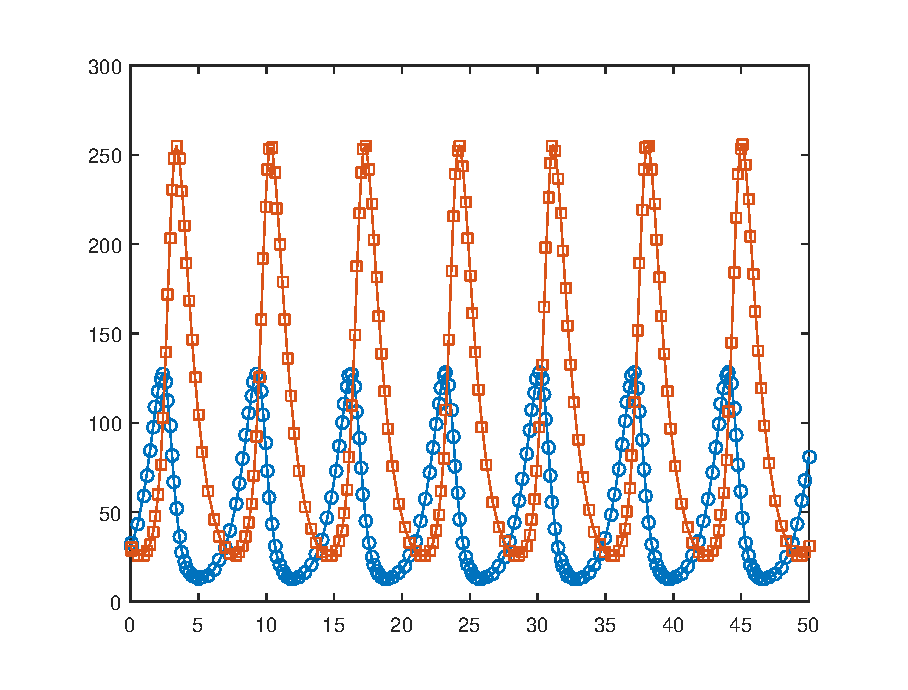
\includegraphics[scale=0.5]{lotka1.eps}
	\caption{Soluci\'on al sistema de Lotka-Volterra con $\alpha = 0.1$, $\beta = 0.02$, $\gamma = 0.1$, $\delta = 0.02$ y condiciones iniciales $S(0) = 30$, $W(0) = 30$.}
	\label{lotka1}
\end{figure}

\begin{figure}
	\centering
	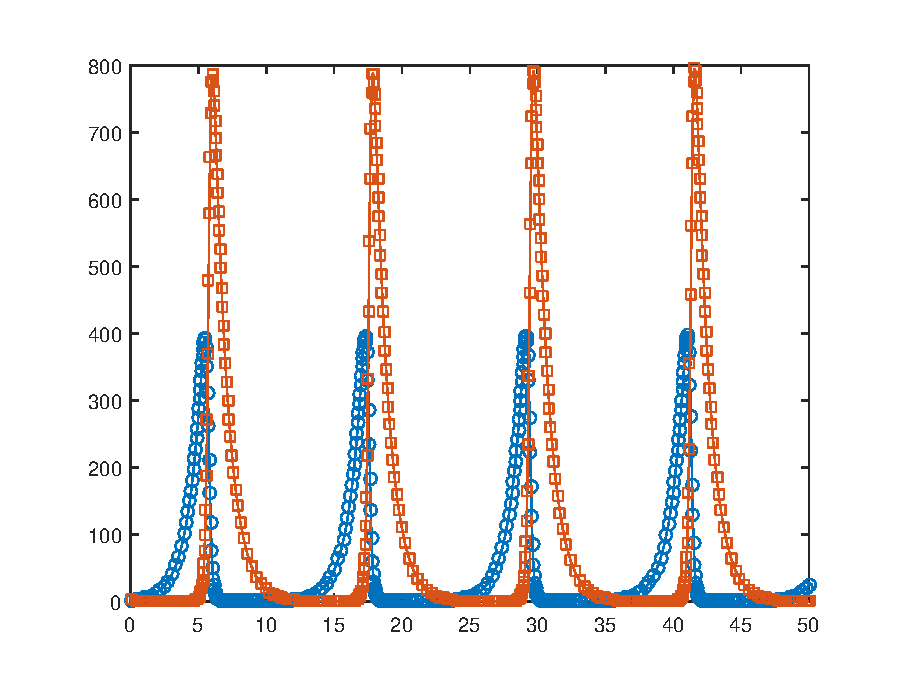
\includegraphics[scale=0.5]{lotkac.eps}
	\caption{Soluci\'on al sistema de Lotka-Volterra con $\alpha = 2$, $\beta = 2$, $\gamma = 2$, $\delta = 1$ y condiciones iniciales $S(0) = 2$, $W(0) = 3$.}
	\label{lotkac}
\end{figure}

Se observa que las soluciones al sistema, esto es, las poblaciones de ambas especies, presentan un comportamiento peri\'odico.

\section{Simulaci\'on}
\label{sec:sim}

El objetivo es realizar dos simulaciones, una para la din\'amica entre las especies lobo-oveja y otra donde se incluya el alimento de las ovejas, esto es, una simulaci\'on para la din\'amica lobo-oveja-pasto.

\subsection{Lobos-Ovejas}
\label{subsec:lo}

En esta versi\'on se cosidera unicamente la interacci\'on entre lobos y ovejas, la poblaci\'on inicial total se fija en $n=60$. 

La simulaci\'on funciona de la siguiente manera: de manera aleatoria se determina la cantidad de individuos que habr\'a de cada especie en el estado inicial, ambas especies se mueven de manera aleatoria en una pradera que queda determinada por el cuadrado unitario. A cada lobo se le asigna una energ\'ia que tambi\'en se determina de manera aleatoria en el conjunto $\{1, ..., 5\}$. 

En cada iteraci\'on en el tiempo, para cada lobo se calcula la distancia $d$ con las ovejas, si $d \leq r$ la oveja muere; $r$ radio de alimentaci\'on de los lobos. Si el lobo come, gana energ\'ia de lo contrario la pierde en la mitad de una unidad.

En el caso de las ovejas, se supone que tienen alimento infinito, por lo que no ganan ni pierden energ\'ia. Su muerte se ve afectada por los lobos y de acuerdo a una probabiblidad $p_{mo}$.

Se permite la reproducci\'on de ambas especies con una probabilidad fija, $p_{rl}$ en el caso de los lobos y $p_{ro}$ en el caso de las ovejas. %Si la poblaci\'on de ovejas es nula, la probabilidad de reproduci\'on de lobos disminuir\'a con el paso del tiempo.

Adem\'as de la muerte por falta de alimento, los lobos mueren de forma natural con una probabilidad fija $p_{ml}$. 

\subsection{Pasto}
\label{subsec:pasto}

Con el objetivo de hacer m\'as realista la simulaci\'on se propone una modificaci\'on: limitar el alimento de las ovejas, de esta forma las ovejas tambi\'en tendr\'an energ\'ia que aumentar\'a o disminuir\'a dependiendo del consumo de alimento. 

La pradera se implementa como un aut\'omata celular. Se trabaja con una malla de 10 $\times$ 10. La supervivencia de cada celda se determinar\'a de acuerdo a las celdas vecinas y la cantidad de ovejas sit\'uan en la misma. En la figura \ref{pasto} se muestra el comportamiento que tiene el aut\'omata de acuerdo a las reglas establecidas.

\begin{figure}[htbp]
\centering
\subfigure[Inicio]{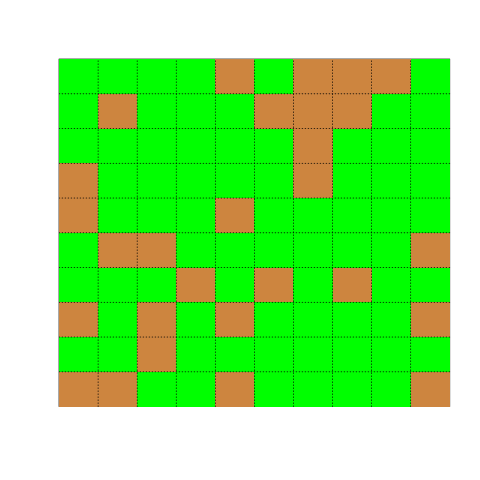
\includegraphics[scale=0.2]{pasto-00.png}}
\subfigure[Paso1]{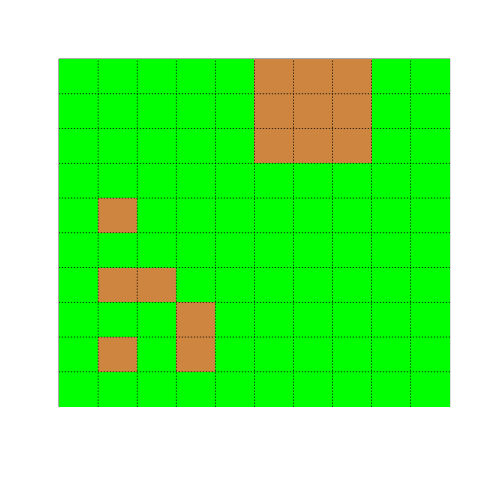
\includegraphics[scale=0.2]{pasto-01.png}}
\subfigure[Paso2]{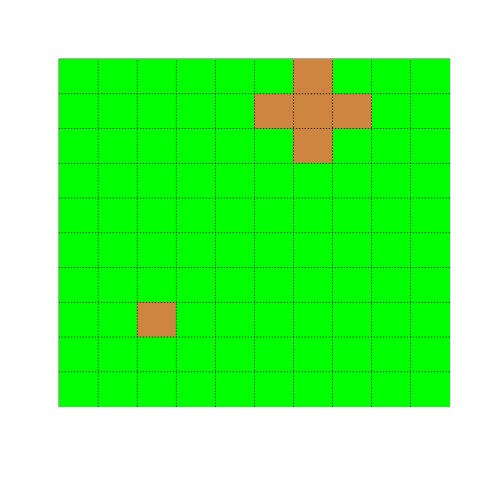
\includegraphics[scale=0.2]{pasto-02.png}}
\subfigure[Paso3]{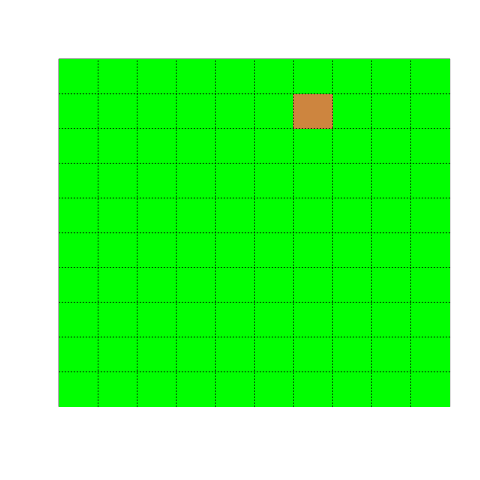
\includegraphics[scale=0.2]{pasto-03.png}}
\caption{Comportamiento de la pradera.} 
\label{pasto}
\end{figure}

\section{Resultados}
\label{sec:resul}

La din\'amica del ecosistema depende de diversos factores tales como las condiciones iniciales, la probabilidad de reproducci\'on y muerte de ambas especies y el radio de alimentaci\'on.

Se realizaron varias pruebas para observar los efectos de algunos de estos factores. En el caso de las condiciones iniciales, se var\'ia la poblaci\'on de lobos dejando los de\'as par\'ametros fijos. Para cada variaci\'on en la poblaci\'on inicial se realizaron 10 r\'eplicas. La figura \ref{ovejas} podemos observar un comportamiento que es de esperarse, mientras aumente la cantidad de lobos en la poblaci\'on inicial, la poblaci\'on de ovejas disminuir\'a.

\begin{figure}
	\centering
	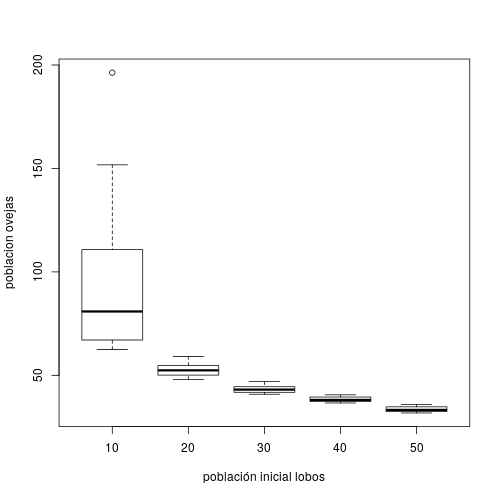
\includegraphics[scale=0.45]{ovejitas.png}
	\caption{Variaci\'on en el promedio de la poblaci\'on de ovejas de acuerdo a la cantidad de lobos en la poblaci\'on inicial.}
	\label{ovejas}
\end{figure}
 
\section{Conclusiones}
\label{sec:con}

El sistema de ecuaciones no representa de manera eficaz la realidad del ecosistema ya que tiene muchas simpleficaciones. El enfoque del sistema multiagente permite simular de manera m\'as realista la din\'amica del sistema.

Se pueden realizar varias mejorar con el fin de aumentar el realismo en la simulaci\'on: a\~nadir sexo a los agentes para que la reproducci\'on se de de la forma correcta, velocidad de movimiento que dependa de la especie, considerar distintos n\'ucleos en el pasto, entre otras.

\bibliographystyle{plain}
\bibliography{bibliop}
\markboth{}{Referencias}
\nocite{*}

\end{document}